\documentclass[11pt]{article}
\usepackage[a4paper,left=1.5cm,right=1.5cm,top=1.5cm,bottom=1.5cm]{geometry}
\usepackage{fancyhdr}
\usepackage{mleftright}
\usepackage{verbatim}
\renewcommand{\headrulewidth}{1pt}
\fancyhead[C]{\textsc{[LINMA2380] --- Homework 4}}
\fancyhead[L]{14 December 2020}
\fancyhead[R]{Group 02}

\usepackage[T1]{fontenc}
\usepackage[utf8]{inputenc}
\usepackage[english]{babel}
\usepackage{graphicx}
\usepackage{subcaption}
\usepackage{csquotes}
\usepackage{mathtools,amssymb,amsthm}
\usepackage[binary-units=true,separate-uncertainty = true,multi-part-units=single]{siunitx}
\usepackage{float}
\usepackage[linktoc=all]{hyperref}
\hypersetup{breaklinks=true}
\graphicspath{{img/}}
\usepackage{caption}
\usepackage{textcomp}
\usepackage{array}
\usepackage{color}
\usepackage{tabularx,booktabs}
\usepackage{titlesec}
\pagestyle{fancy}
\usepackage{mathrsfs}
\usepackage{bm}
\usepackage[ruled,linesnumbered]{algorithm2e}
\usepackage{tikz}
\usetikzlibrary{matrix}
\usetikzlibrary{calc}
\usetikzlibrary{fit}

\newtheorem{theorem}{Theorem}[section]
\newtheorem{corollary}{Corollary}[theorem]
\newtheorem*{lemma}{Lemma}

\DeclarePairedDelimiterX{\norm}[1]{\lVert}{\rVert}{#1}

\newcommand\bovermat[2]{%
  \makebox[0pt][l]{$\smash{\overbrace{\phantom{%
    \begin{matrix}#2\end{matrix}}}^{\text{#1}}}$}#2}
    
\newcommand{\imag}{\mathrm{i}\mkern1mu} % Imaginary unit
\newcommand{\abs}[1]{\left\lvert#1\right\lvert}
\newcommand{\kp}{\otimes}
\DeclareMathOperator{\vect}{vec}

\DeclareMathOperator*{\argmin}{arg\,min}

\DeclareMathOperator{\rank}{rank}
\DeclareMathOperator{\Ker}{Ker}
\DeclareMathOperator{\newdiff}{d} % use \dif instead
\newcommand{\dif}{\newdiff\!}
\newcommand{\e}{\mathrm{e}}
\newcommand{\bo}{\mathcal{O}}

\DeclareMathOperator{\diag}{diag}

\newcommand{\field}{\mathbb{F}} % field
\newcommand{\real}{\mathbb{R}} % real numbers
\newcommand{\complex}{\mathbb{C}} % complex numbers

\newcommand{\snorm}[1]{\norm{#1}_2} % spectral norm
\newcommand{\fnorm}[1]{\norm{#1}_F} % frobenius norm

\setcounter{MaxMatrixCols}{15}

\newcommand\undermat[2]{% http://tex.stackexchange.com/a/102468/5764
	\makebox[0pt][l]{$\smash{\underbrace{\phantom{%
					\begin{matrix}#2\end{matrix}}}_{\text{$#1$}}}$}#2}

\begin{document}
\section*{Exercise A: Minimal polynomial and Smith normal form}
\subsection*{A1}
First we prove a lemma.
\begin{lemma}
 If $A\in\real^{n\times n}$ and $B\in\real^{n\times n}$ then for $k=1,...,n$:
 \begin{itemize}
     \item $\delta_k(A)$ divides $\delta_k(AB)$
     \item $\delta_k(B)$ divides $\delta_k(AB)$
 \end{itemize}
\end{lemma}
\begin{proof}
If we denote by $(AB)_{\textbf{I}\textbf{J}}$ the k-by-k sub-matrix of $AB$ taking the rows $\textbf{I}$ and the columns $\textbf{J}$ (hence $|\textbf{I}|=|\textbf{J}|=k$). We can write and develop the associated k-minor:
\begin{align*}
    \det (AB)_{\textbf{I}\textbf{J}}&=\det(A_{\textbf{I}*}B_{*\textbf{J}})\\
    &=\sum_{\textbf{j}_k} A_{\textbf{I}*}\binom{k}{\textbf{j}_k}B_{*\textbf{J}}\binom{\textbf{j}_k}{k}\\
    &=\sum_{\textbf{j}_k} \det A_{\textbf{I} \textbf{j}_k} \det B_{\textbf{j}_k \textbf{J}}\ \
\end{align*}
The second equality is derived from the Binet-Cauchy theorem. We observe that the k-minors of $AB$ can be written as linear combinations of the k-minors of $A$. Thus, every common divisor of the k-minors of $A$ must also be a common divisor of the k-minors of $AB$. As it is true for the greatest common divisor, we have that $\delta_k(A)$ divides $\delta_k(AB)$. The same reasoning is valid taking $B$ instead of $A$ and therefore we prove that $\delta_k(B)$ divides $\delta_k(AB)$.\\
\end{proof}
We now prove that \(\delta_k\big(P(\lambda)\big) = \delta_k\big(Q(\lambda)\big)\), where \(Q(\lambda) = M(\lambda) P(\lambda) N(\lambda)\).

\begin{proof}
Using the lemma with $A=M(\lambda)P(\lambda)$ and $B=N(\lambda)$, we have that $\delta_k(M(\lambda)P(\lambda))$ divides $\delta_k(Q(\lambda))$. Then applying once more the lemma with $A=\delta_k(M(\lambda))$ and $B=\delta_k(P(\lambda))$, we obtain that $\delta_k(P(\lambda))$ divides $\delta_k(M(\lambda)P(\lambda))$. We deduce that $\delta_k(P(\lambda))$ divides $\delta_k(Q(\lambda))$.\\

We can apply the exact same reasoning to $P(\lambda)=N^{-1}(\lambda)Q(\lambda)M^{-1}(\lambda)$. Doing so, we have that $\delta_k(Q(\lambda))$ divides $\delta_k(P(\lambda))$. Consequently, we conclude that $\delta_k(Q(\lambda))$ is equal to $\delta_k(P(\lambda))$.
\end{proof}

\subsection*{A2}.
We now prove that for all $k\in\{1,...,n\}$, $\delta_k(P(\lambda))=\Pi^k_{i=1}d_i(\lambda)$ where $d_i(\lambda)$ are the diagonal entries of $D(\lambda)$ and $M(\lambda)D(\lambda)N(\lambda)$ is a Smith decomposition of $P(\lambda)$.
\begin{proof}
From A1, we know that $\delta_k(P(\lambda))=\delta_k(D(\lambda))$ and therefore we will consider $\delta_k(D(\lambda))$.\\
We first note that all sub-matrices of $D(\lambda)$ are either triangular inferior, triangular superior or null. The determinants of these sub-matrices are hence given by the product of the diagonal elements. The only sub-matrices for which the determinant is non-zero are these where the indices of the removed rows are identical to the indices of the removed columns. Because 0 has infinitely many divisors, we should therefore only consider the case where this specific case.\\
We denote by $\textbf{j}=(j_1,...,j_k)$, where $j_1<...<j_k$, the indices of the rows and columns that are kept. The determinant associated to $\textbf{j}$ can be written as:
\begin{equation*}
    \det D_{\textbf{j}}(\lambda)=d_{j_1}(\lambda)...d_{j_k}(\lambda)
\end{equation*}
We now use the property that $d_i(\lambda)$ divides $d_{i+1}(\lambda)$ for all $i\in\{1,...,n-1\}$.\\
If we consider the $i$th factor $d_{j_i}(\lambda)$, we observe that $d_i(\lambda)$ divides $d_{j_i}(\lambda)$ as $j_i$ is either equal to $i$ or larger than $i$ (due to the strict inequality $j_1<...<j_k$). Hence $d_{j_i}(\lambda)$ can be rewritten as $a_{j_i}(\lambda)d_i(\lambda)$ for a certain $a_{j_i}(\lambda)\in\complex[\lambda]$. The determinant can thus be developed as:
\begin{equation}\label{detDj}
    \det D_{\textbf{j}}(\lambda)=a_{j_1}(\lambda) d_1(\lambda)...a_{j_k}(\lambda)d_{k}(\lambda)
\end{equation}
We also observe that when $\textbf{j}=(1,...,k)$, we have:
\begin{equation}\label{123}
    \det D_{\textbf{j}}(\lambda)=\Pi_{i=1}^k d_i(\lambda)
\end{equation}
which is a monic polynomial as it is the product of monic polynomials.\\
Because $\Pi_{i=1}^k d_i(\lambda)$ is a divisor of \eqref{detDj} for any $\textbf{j}$ and that $\delta_k(D(\lambda))$ cannot contain any additional factor due to \eqref{123}, we conclude that the monic greatest common divisor of all k-minors of $D(\lambda)$ is $\Pi_{i=1}^k d_i(\lambda)$. Therefore, we have:
\begin{equation}\label{A21}
    \delta_k(P(\lambda))=\delta_k(D(\lambda))=\Pi_{i=1}^k d_i(\lambda)
\end{equation}
\end{proof}
The diagonal entries $d_1(\lambda),...,d_n(\lambda)$ of $D(\lambda)$ are unique and depend only on the sequence $\delta_1(P(\lambda))$,...,$\delta_n(P(\lambda))$.
\begin{proof}
We first consider the first entry $d_1(\lambda)$. From \eqref{A21}, we know that $d_1(\lambda)=\delta_1(\lambda)$. The notion of monic greatest common divisor leads to the unicity of $\delta_1(\lambda)$ and hence we deduce $d_1(\lambda)$ is unique as well. This constitutes the base case of the induction proof.\\
%Next, we show that if $d_1(\lambda)$ is unique then $d_2(\lambda)$ is unique as well. From \eqref{A21}, we have $d_2(\lambda)=\delta_2(\lambda)/d_1(\lambda)$. This implies $d_2(\lambda)$ is unique as the notion of monic greatest common divisor implies the unicity of $\delta_2(\lambda)$ and $d_1(\lambda)$ is unique.
Next, we prove that if $d_k(\lambda)$ is unique then $d_{k+1}(\lambda)$ is also unique. Again from \eqref{A21}, we have that $d_{k+1}(\lambda)=\delta_{k+1}(P(\lambda))/d_k(\lambda)$. By the unicity of the notion of monic greatest common divisor and the unicity $d_k(\lambda)$, we conclude that $d_{k+1}(P(\lambda))$ is unique.\\
Clearly the diagonal entries $d_1(\lambda),...,d_n(\lambda)$ can be computed using the sequence $\delta_1(P(\lambda)),...,\delta_n(P(\lambda))$. First, we have $d_1(\lambda)=\delta_1(P(\lambda))$ and then we use $d_{k+1}(\lambda)=\delta_{k+1}(P(\lambda))/ d_k(\lambda)$ for the next entries.
\end{proof}
There are unimodular matrices $M(\lambda),N(\lambda)\in\complex^{n\times n}[\lambda]$ such that $Q(\lambda)=M(\lambda)P(\lambda)N(\lambda)$ if and only if $\delta_k(P(\lambda))=\delta_k(Q(\lambda))$ for all $k\in\{1,...,n\}$.
\begin{proof}
$\Rightarrow$ This was shown in A1.\\
$\Leftarrow$
From the previous proved statement we know that the diagonal entries of $D(\lambda)$ of the Smith decomposition of $P(\lambda)$ are unique and depend only on the sequence $\delta_1(P(\lambda)),...,\delta_n(P(\lambda))$. As this sequence is the same for $P(\lambda)$ and $Q(\lambda)$, we deduce $D(\lambda)$ is the same for their Smith decompositions:
% does the smith decomposition exist for every matrix ?
\begin{align*}
    P(\lambda)&=M_1(\lambda) D(\lambda) N_1(\lambda)\\
    Q(\lambda)&=M_2(\lambda) D(\lambda) N_2(\lambda)
\end{align*}
where $M_1(\lambda),M_1(\lambda),M_1(\lambda),M_1(\lambda)\in\complex^{n\times n}[\lambda]$ are unimodular and $D(\lambda)\in\complex^{n\times n}[\lambda]$ diagonal.\\
From the first equation, we can write $D(\lambda)=M_1(\lambda)^{-1} P(\lambda) N_1(\lambda)^{-1}$ as $M_1(\lambda)$ and $N_1(\lambda)$ are unimodular and hence invertible. Next, we inject this expression of $D(\lambda)$ in the second equation and we obtain:
\begin{equation*}
    Q(\lambda)=M_2(\lambda) M_1(\lambda)^{-1} P(\lambda) N_1(\lambda)^{-1} N_2(\lambda)
\end{equation*}
Finally, as the inverse of a unimodular matrix is unimodular and the product of unimodular matrices is unimodular, we have $M(\lambda)=M_2(\lambda) M_1(\lambda)^{-1}$ and $N(\lambda)=N_1(\lambda)^{-1} N_2(\lambda)$ which are unimodular matrices such that $Q(\lambda)=M(\lambda)P(\lambda)N(\lambda)$.

\end{proof}

\subsection*{A3}
Let $A\in \complex^{n\times n}$ be a Jordan block with eigenvalue $\lambda_1$. The elementary polynomials of $\lambda I-A$ are equal to: $d_i(\lambda)=1$ for $i=1,...,n-1$ and $d_n(\lambda)=(\lambda-\lambda_1)^n$.
\begin{proof}
We first write the matrix $\lambda I-A$ that we call $P(\lambda)$:
\begin{equation*}
    P(\lambda)=\lambda I-A=
    \begin{pmatrix}
    \lambda-\lambda_1 & -1 & & \\
    & \ddots & \ddots & \\
    & & \ddots & -1\\
    & & & \lambda-\lambda_1 \\
    \end{pmatrix}
\end{equation*}
As we have seen the sequence $d_1(\lambda),...,d_n(\lambda)$ can be derived by the sequence $\delta_1(P(\lambda)),...,\delta_n(P(\lambda))$, we first derive the latter sequence. When computing each $\delta_k(P(\lambda))$, we observe that for $k<n$, a valid sub-matrix to take into account is the one which has all the $-1$ entries on its diagonal. We illustrate here the case where $k=n-1$:
\[P(\lambda) = 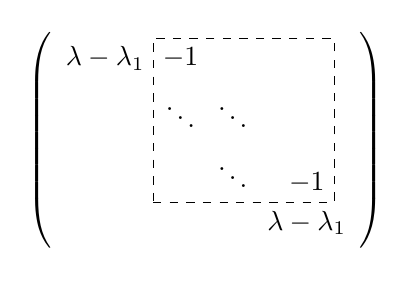
\begin{tikzpicture}[baseline=(math-axis),every right delimiter/.style={xshift=-3pt},every left delimiter/.style={xshift=3pt}]%
\matrix [matrix of math nodes,left delimiter=(,right delimiter=)] (matrix)
{
|(m11)| \lambda-\lambda_1 & |(m12)| -1 & |(m13)| & |(m14)|\\
|(m21)| & |(m22)| \ddots & |(m23)| \ddots & |(m24)| \\
|(m31)| & |(m32)| & |(m33)| \ddots & |(m34)| -1\\
|(m41)| & |(m42)| & |(m43)| & |(m44)| \lambda-\lambda_1\\
};
\node[draw,dashed,inner sep=0pt,fit=(m12) (m14) (m32) (m34)] {};
\coordinate (math-axis) at ($(matrix.center)+(0em,-0.25em)$);
\end{tikzpicture}\]
As this sub-matrix is triangular inferior, its determinant is equal to the product of its diagonal entries. The determinant of such matrices is therefore 1 or -1. As 1 and -1 have only one monic divisor which is 1, we conclude that $\delta_k(P(\lambda))=1$ for $k\in\{1,...,n-1\}$. From the recursive formula proposed in A2, we deduce that $d_k(\lambda)=1$ for $k\in\{1,...,n-1\}$.\\
When $k=n$, the only possible sub-matrix to consider is the whole matrix which determinant is equal to the product of the diagonal entries, hence $(\lambda-\lambda_1)^n$. We deduce that $\delta_n(P(\lambda))=(\lambda-\lambda_1)^n$ and therefore using the recursive formula proposed in A2 we obtain $d_n(\lambda)=(\lambda-\lambda_1)^n$.
\end{proof}

\subsection*{A4}
Let $J_1 \in \mathbb{C}^{n_1 \times n_1}$ and $J_2 \in \mathbb{C}^{n_2 \times n_2}$ be two Jordan blocks with respective eigenvalues $\lambda_i$ and size $n_i$, $i = 1,2$. Let $A\in \mathbb{C}^{n\times n}$ with $n = n_1+n_2$ be the Jordan matrix consisting of the two Jordan blocks $J_1$ and $J_2$. Then $\lambda I - A$ can be reduced to the form
\[
M(\lambda) (\lambda I-A)N(\lambda) = diag\{\underbrace{1, \dots , 1}_{n_1 - 1}, (\lambda - \lambda_1)^{n_1}, \underbrace{1, \dots, 1}_{n_2 - 1}, (\lambda - \lambda_2)^{n_2}\}
\]
With unimodular matrices  $M(\lambda)$, $N(\lambda) \in \mathbb{C}^{n\times n}[\lambda]$.

\begin{proof}
From A3, we have already proved that $\lambda I - J_1$ can be written as
\begin{align*}
P_1(\lambda) &:= \lambda I_{n_1} - J_1 = M_1(\lambda) D_1(\lambda) N_1(\lambda)\\
\Leftrightarrow D_1 &= M_1^{-1}(\lambda)P_1(\lambda) N_1^{-1}(\lambda)\\
&= \begin{bmatrix}
1 & & & &\\
  &1& & &\\
  & &\ddots& &\\
  & & & 1& \\
  & & &  &(\lambda - \lambda_1)^{n_1}\\
\end{bmatrix}
\end{align*} 

Similarly, 
\begin{align*}
P_2(\lambda) &:= \lambda I_{n_2} - J_2 = M_2(\lambda) D_2(\lambda) N_2(\lambda)\\
\Leftrightarrow D_2 &= M_2^{-1}(\lambda)P_2(\lambda) N_2^{-1}(\lambda)\\
&= \begin{bmatrix}
1 & & & &\\
  &1& & &\\
  & &\ddots& &\\
  & & & 1& \\
  & & &  &(\lambda - \lambda_2)^{n_2}\\
\end{bmatrix}
\end{align*}

Note that $M_1^{-1}(\lambda)$, $N_1^{-1}(\lambda)$, $M_2^{-1}(\lambda)$ and $N_2^{-1}(\lambda)$ are unimodular as their inverse are unimodular.

Now, if we consider the diagonal matrix formed by $D_1$ and $D_2$, we have :
\begin{align*}D(\lambda):=
\begin{bmatrix}
D_1 &\\
& D_2
\end{bmatrix} &= \begin{bmatrix}
1 & & & &&&&&\\
  &1& & &&&&&\\
  & &\ddots& &&&&&\\
  & & & 1& &&&&\\
  & & &  &(\lambda - \lambda_1)^{n_1}&&&&\\
  &&&&&1 & & & &\\
  &&&&&&1& & &\\
  &&&&&& &\ddots& &\\
  &&&&&& & & 1& \\
  &&&&&&& &  &(\lambda - \lambda_2)^{n_2}\\
\end{bmatrix}\\
&=\begin{bmatrix}
M_1^{-1}(\lambda)P_1(\lambda) N_1^{-1}(\lambda) &\\
& M_2^{-1}(\lambda)P_2(\lambda) N_2^{-1}(\lambda)
\end{bmatrix}\\
&=
\underbrace{\begin{bmatrix}
M_1^{-1}(\lambda) &\\
& M_2^{-1}(\lambda)
\end{bmatrix}}_{:=M(\lambda)}
\underbrace{\begin{bmatrix}
P_1\lambda) &\\
& P_2(\lambda)
\end{bmatrix}}_{:= P(\lambda) = (\lambda I - A)}
\underbrace{\begin{bmatrix}
N_1^{-1}(\lambda) &\\
& N_2^{-1}(\lambda)
\end{bmatrix}}_{:=N(\lambda)}
\end{align*}

$M(\lambda)$ is indeed unimodular as its determinant is the product of the determinants of $M_1^{-1}(\lambda)$ and $M_2^{-1}(\lambda)$ (both unimodular). Thus, the determinant of $M_1(\lambda)$ is equal to the product of 2 nonzero constants, which is a nonzero constant.

Similarly, $N(\lambda)$ is also unimodular.
\end{proof}
\textbf{Remark} : this result can be easily extended to the case of A being composed by more than 2 Jordan blocks with the same reasoning. 
\footnotesize{
\begin{align}
\underbrace{\begin{bmatrix}
D_1 & & & \\
& D_2 & & \\
& & D_3 & \\
& & & & \ddots
\end{bmatrix} }_{:= D(\lambda)}
&=
\underbrace{\begin{bmatrix}
M_1^{-1}(\lambda) & & &\\
& M_2^{-1}(\lambda) & &\\
& & M_3^{-1}(\lambda) & \\
& & & \ddots
\end{bmatrix}}_{:=B^{-1}(\lambda)}
\underbrace{\begin{bmatrix}
P_1\lambda) & & &\\
& P_2(\lambda) & &\\
& & P_3(\lambda) &\\
& & & \ddots
\end{bmatrix}}_{:= P(\lambda) = (\lambda I - A)}
\underbrace{\begin{bmatrix}
N_1^{-1}(\lambda) & & &\\
& N_2^{-1}(\lambda) & &\\
& & N_3^{-1}(\lambda) & \\
& & & \ddots
\end{bmatrix}}_{:=C^{-1}(\lambda)}
\end{align}\label{a4}}
\normalsize
\begin{proof}
By induction, let's consider $A=\begin{bmatrix}
A_1 & \\
 & J_p
\end{bmatrix}$. With $A_1 \in \mathbb{C}^{n\times n}$ a block diagonal matrix with $(p-1)$ Jordan blocks and $J_p\in \mathbb{C}^{m\times m}$ the pth Jordan block. 
We have already proved the case $p = 2$.

For $p > 2$, let's assume that :
\footnotesize{
\begin{align*}
\underbrace{\begin{bmatrix}
D_1 & & & \\
& D_2 & & \\
& & \ddots & \\
& & & & D_{p-1}
\end{bmatrix} }_{:= D_{A_1}(\lambda)}
&=
\underbrace{\begin{bmatrix}
M_1^{-1}(\lambda) & & &\\
& M_2^{-1}(\lambda) & &\\
& & \ddots & \\
& & & M_{p-1}^{-1}(\lambda)
\end{bmatrix}}_{:=M_{A_1}^{-1}(\lambda)}
\underbrace{\begin{bmatrix}
P_1\lambda) & & &\\
& P_2(\lambda) & &\\
& &\ddots &\\
& & &  P_{p-1}(\lambda)
\end{bmatrix}}_{:= P_{A_1}(\lambda) = (\lambda I - A_1)}
\underbrace{\begin{bmatrix}
N_1^{-1}(\lambda) & & &\\
& N_2^{-1}(\lambda) & &\\
& & N_3^{-1}(\lambda) & \\
& & & \ddots
\end{bmatrix}}_{:=N_{A_1}^{-1}(\lambda)}
\end{align*}}
 \normalsize
 
 Then, 
 \begin{align*}
 \lambda I_{m+n} - A &= \begin{bmatrix}
 \lambda I_{n} - A_1 & \\
  & \lambda I_{m} - J_p 
 \end{bmatrix}\\
 &= \begin{bmatrix}
 M_{A_1}(\lambda) D_{A_1}(\lambda) N_{A_1}(\lambda) & \\
 & \lambda I_{m} - J_p 
 \end{bmatrix}\\
  &= \begin{bmatrix}
 M_{A_1}(\lambda) D_{A_1}(\lambda) N_{A_1}(\lambda) & \\
 & M_{J_p}(\lambda) D_{J_p}(\lambda) N_{J_p}(\lambda)
 \end{bmatrix}\\
 &= \underbrace{\begin{bmatrix}
 M_{A_1}(\lambda) & \\
  & M_{J_p}(\lambda)
 \end{bmatrix}}_{B(\lambda)}\underbrace{\begin{bmatrix}
 D_{A_1}(\lambda) & \\
  & D_{J_p}(\lambda)
 \end{bmatrix}}_{D(\lambda)}\underbrace{\begin{bmatrix}
 N_{A_1}(\lambda) & \\
  & N_{J_p}(\lambda)
 \end{bmatrix}}_{C(\lambda)}
 \end{align*}
 From the first equation to the second, we used our assumption and from the second to the third, we used A3.

\end{proof}

Now, we want to find the elementary polynomials of $P(\lambda) = (\lambda I - A)$. For that, we will use the property proved in A1 s.t. $\delta_k(P(\lambda)) = \delta_k(D(\lambda))$.

Indeed, it is clear that for $k =1, 2, \dots,(n_1 + n_2 - 2)$, we can always choose a submatrix containing only ones on the diagonal, which means that $\delta_k(P(\lambda)) = 1$ . And by A2, we have that the monic $d_k(\lambda)$ are all equal to 1 for $k =1, 2, \dots, (n_1 + n_2 - 2)$. 

Then, we need to distinguish 2 cases : 
\begin{itemize}
\item When $\lambda_1 \neq \lambda_2$, \begin{align*}
&\delta_{n_1+n_2 - 1}(P(\lambda)) = 1  &\Leftrightarrow& d_{n_1+n_2-1}(\lambda) = 1\\
&\delta_{n_1+n_2}(P(\lambda)) = (\lambda -\lambda_{1})^{n_1}(\lambda -\lambda_{2})^{n_2} &\Leftrightarrow& d_{n_1+n_2}(\lambda) = (\lambda -\lambda_{1})^{n_1}(\lambda -\lambda_{2})^{n_2}
\end{align*}
\item When $\lambda_1 = \lambda_2$, \begin{align*}
&\delta_{n_1+n_2 - 1}(P(\lambda)) = (\lambda -\lambda_{1})^{\min(n_1,n_2)} &\Leftrightarrow& d_{n_1+n_2-1}(\lambda) = (\lambda -\lambda_{1})^{\min(n_1,n_2)}\\
&\delta_{n_1+n_2}(P(\lambda)) = (\lambda -\lambda_{1})^{n_1+n_2} &\Leftrightarrow& d_{n_1+n_2}(\lambda) = \frac{(\lambda -\lambda_{1})^{n_1+n_2}}{(\lambda -\lambda_{1})^{\min(n_1,n_2)}}=(\lambda -\lambda_{1})^{\max(n_1,n_2)}
\end{align*}
\end{itemize}

We can observe that the minimal polynomial of $A$ is equal to $d_{n_1+n_2}(\lambda)$.

~\\
\textbf{Remark} : This equality is also valid if A has more than 2 Jordan blocks.

\begin{proof}
By induction, let's consider $A=\begin{bmatrix}
A_1 & \\
 & J_p
\end{bmatrix}$. With $A_1 \in \mathbb{C}^{n\times n}$ a block diagonal matrix with $(p-1)$ Jordan blocks and $J_p\in \mathbb{C}^{m\times m}$ the pth Jordan block. 
We have already proven the case $p = 2$.

For $p > 2$, let's assume that the minimal polynomial of $A_1$ is equal to the last elementary polynomial of $(\lambda I - A_1)$: $d_{n}^{A_1}(\lambda) = \prod_{i = 1}^k (\lambda - \lambda_i)^{m_i}$. With $\lambda_i$, $i= 1 \dots k$, the distinct eigenvalues of A and $m_i$ the size of the largest Jordan block associated to the corresponding eigenvalue.

We know that
\begin{align*}
 P(\lambda):=\lambda I_{m+n} - A 
&= \underbrace{\begin{bmatrix}
 M_{A_1}(\lambda) & \\
  & M_{J_p}(\lambda)
 \end{bmatrix}}_{B(\lambda)}\underbrace{\begin{bmatrix}
 D_{A_1}(\lambda) & \\
  & D_{J_p}(\lambda)
 \end{bmatrix}}_{D(\lambda)}\underbrace{\begin{bmatrix}
 N_{A_1}(\lambda) & \\
  & N_{J_p}(\lambda)
 \end{bmatrix}}_{C(\lambda)}
 \end{align*}
 
 So $\delta_{n+m}(P(\lambda)) = \delta_{n+m}(D(\lambda)) = \prod_{i = 1}^p (\lambda - \lambda_i)^{x_i}$ with $p$ the total number of Jordan blocks and $x_i$ the size of each Jordan block.
 
 Now, let's consider 2 cases.
 \begin{itemize}
 \item If $\lambda_p \neq \lambda_i , \forall i\neq p$, then $(\lambda - \lambda_p)^{x_p}$ is not a divisor of any i-minor with $i < (n+m)$. Which means that $d_{n+m}(\lambda) = d_{n}^{A_1}(\lambda) (\lambda - \lambda_p)^{x_p}$. This corresponds to the minimal polynomial of A.
 \item If $\exists i : \lambda_p = \lambda_i$, then let's denote $y$ as the number of Jordan blocks with an eigenvalue equal to $\lambda_p$. It is clear that if we choose any submatrix of dimension $(n+m-y+1)$, there will be at least one occurence of $(\lambda - \lambda_p)^{z}$ (with $ z \in \mathcal{Z}_p$, $\mathcal{Z}_p$ is the set of all sizes of Jordan blocks with eigenvalue equal to $\lambda_p$). Which means that $\delta_{n+m-y+1} (P(\lambda))$ is divisible by $(\lambda - \lambda_p)^{\min(\mathcal{Z}_p)}$ and so is $d_{n+m-y+1}^{A}(\lambda)$. We can continue with this reasoning by considering  $\tilde{\mathcal{Z}}_p =  \mathcal{Z}_p \setminus \min(\mathcal{Z}_p)$ and submatrices of dimension $(n+m-y+2)$... When we arrive at the dimension $(n+m)$, it is logical that $d_{n+m}^{A}(\lambda) = \frac{\delta{n+m}(P(\lambda))}{\prod_{z \in \mathcal{Z}_p\setminus \max{(\mathcal{Z}_p)}}(\lambda - \lambda_p)^{z}}$. Which means that the only contribution of $\lambda_p$ in $d_{n+m}^{A}(\lambda)$ is $(\lambda - \lambda_p)^{\max(\mathcal{Z}_p)}$. And so, from $d_{n+m}^{A_1}(\lambda)$, we take out the factor with $\lambda_p$ in it and we replace it with the new $(\lambda - \lambda_p)^{\max(\mathcal{Z}_p)}$. With this, we obtain the minimal polynomial of A.
 \end{itemize}
\end{proof}
\subsection*{A5}
Let $A\in \mathbb{C}^{n\times n}$. There are unimodular matrices $M(\lambda), N(\lambda) \in \mathbb{C}^{n\times n}[\lambda]$ s.t. 
\[\lambda I - A = M(\lambda)E(\lambda)N(\lambda)
\] where $E(\lambda)$ is diagonal with elements being either 1's or polynomials of the form $(\lambda - \lambda_i)^{n_i}$ where $ \lambda_i$ are the eigenvalues of A and $n_i$ the size of the corresponding Jordan block in the Jordan decomposition of A.

\begin{proof}
First, let us write the Jordan decomposition of A.
\[T^{-1} A T =J \qquad \Leftrightarrow \qquad A= T J T^{-1}
\]

With $J$, the Jordan matrix and $T$ being a similarity transformation (this implies that $T$ is invertible, its determinant is nonzero, which means that it is a unimodular matrix).

We can now derive :
\begin{align*}
\lambda I - A &= \lambda I - T J T^{-1}\\
&= T(\lambda I - J) T^{-1}\\
&= \underbrace{TB(\lambda)}_{:=M(\lambda)}\underbrace{D(\lambda)}_{:= E(\lambda)}\underbrace{C(\lambda)T^{-1}}_{:= N(\lambda)}
\end{align*}
The last equality is obtained with the results in A4 (cfr Equation \ref{a4}). 
$M(\lambda)$ and $N(\lambda)$ are indeed unimodular as they are products of 2 unimodular matrices.
\end{proof}

The matrices $A$ and $J$ have the same eigenvalues which means that they have the same minimal polynomial as well. In A4, we have already observed that a Jordan matrix has a minimal polynomial equal to its last elementary polynomial.

Hence the minimal polynomial of $A$ is equal to the last elementary polynomial of $J$ (obtained with $D(\lambda)$) which is also the last elementary polynomial of $A$ (obtained with $E(\lambda) = D(\lambda)$). 
\section*{Exercise B: Implementation}
\subsection*{B1}
Using the Jordan normal form is not numerically stable because taking limits does not commute with forming the Jordan canonical form.
A simple example is the matrix \(A = I_2\), approximated by \(A_\varepsilon = \left[\begin{smallmatrix} 1 & \varepsilon \\ 0 & 1\end{smallmatrix}\right]\), the latter having Jordan canonical form \(J_\varepsilon = \left[\begin{smallmatrix} 1 & 1 \\ 0 & 1\end{smallmatrix}\right]\).
However, the Jordan form of \(A\) is simply \(J = I_2\).
We thus have
\[
\lim_{\varepsilon \to 0} A_\varepsilon = A, \quad \textnormal{but} \quad \lim_{\varepsilon \to 0} J_\varepsilon \neq J.
\]
Similarly, computing the minimal polynomials yields \(p_{A_\varepsilon}(\lambda) = (\lambda - 1)^2 \ne \lambda - 1 = p_A(\lambda)\).

\subsection*{B2}
We want to compute the Smith normal form of $\lambda I - A_{i}$ where $A_{i}$ is one of the three matrices: $A_1$, $A_2$ and $A_3$ defined in the homework statement. The Smith normal forms are the following:

\begin{align*} P(\lambda I - A_{1}) &=
    \begin{pmatrix}
    1 & 0 & 0 & 0 \\
    0 & 1 & 0 & 0 \\
    0 & 0 & 1 & 0 \\
    0 & 0 & 0 & \lambda^{4} + 4 \lambda^{3} + \frac{21 \lambda^{2}}{4} + \frac{11 \lambda}{4} + \frac{1}{2}
    \end{pmatrix} \\
    P(\lambda I - A_{2}) &=
    \begin{pmatrix}
    1 & 0 & 0 & 0 \\
    0 & 1 & 0 & 0 \\
    0 & 0 & 1 & 0 \\
    0 & 0 & 0 & \lambda^{4} + \frac{7 \lambda^{3}}{2} + \frac{7 \lambda^{2}}{2} + \lambda
    \end{pmatrix} \\
    P(\lambda I - A_{3}) &=
    \begin{pmatrix}
    1 & 0 & 0 & 0 \\
    0 & 1 & 0 & 0 \\
    0 & 0 & 1 & 0 \\
    0 & 0 & 0 & \lambda^{4} + 3 \lambda^{3} + 2 \lambda^{2}
    \end{pmatrix}
\end{align*}

The minimal polynomial of $A_{i}$ can be deduced from the last elementary polynomial of those Smith normal forms.

\begin{align*}
    m_{1}(\lambda) &= \lambda^{4} + 4 \lambda^{3} + \frac{21 \lambda^{2}}{4} + \frac{11 \lambda}{4} + \frac{1}{2} \\
    &= \frac{1}{4} (\lambda + 2) (\lambda + 1) (2 \lambda + 1)^{2} \\
    m_{2}(\lambda) &= \lambda^{4} + \frac{7 \lambda^{3}}{2} + \frac{7 \lambda^{2}}{2} + \lambda \\
    &= \frac{1}{2} \lambda (2 \lambda + 1) (\lambda + 2) (\lambda + 1) \\
    m_{3}(\lambda) &= \lambda^{4} + 3 \lambda^{3} + 2 \lambda^{2} \\
    &= \lambda^{2} (\lambda + 2) (\lambda + 1)
\end{align*}

We want to test the boundednesss of the trajectories defined by the systems with the three different matrices: $A_1$, $A_2$ and $A_3$ defined in the homework statement. For this purpose, we use statement 2 in the introduction of exercise A of the homework 3: " All the eigenvalues of $A_{i}$ are in the open left-hand plane, or are on the imaginary axis and are simple." because it has been shown as equivalent to statement 1 ("Every trajectory of $\dot{x}(t) = A x(t), x(t) \in \complex^{n}, t\geq 0$ is bounded: $\forall x(0) \in \complex^{n}, sup_{t\geq0} \norm{x(t)} < \infty$") in the homework 3 .

To check whether statement 2 is satisfied or not, we looked at the vectors of eigenvalues $\Lambda_i$ of the matrices which are computed from the factorization of the minimal polynomial.
\begin{align*}
    \Lambda_1 =\begin{pmatrix}
    -0.5\\
    -0.5\\
    -1\\
    -2
    \end{pmatrix},
    \Lambda_2 =\begin{pmatrix}
    0\\
    -0.5\\
    -1\\
    -2
    \end{pmatrix},
    \Lambda_3 =\begin{pmatrix}
    0\\
    0\\
    -1\\
    -2
    \end{pmatrix}.
\end{align*}
We observe that the eigenvalues are identical to the eigenvalues found in the homework 3. The conclusion is thus similar: all eigenvalues of $A_1$ (for all \(i\)) are such that $\Re(\lambda_{1, i})<0$.$A_1$ hence satisfies statement 2.
The matrix $A_2$ has eigenvalues such $\Re(\lambda_{2, i})<0$ for all \(i\) except for ($\lambda_{21}=0$), which is simple (the multiplicity of this eigenvalue in the factorization of the minimal polynomial is one), so the statement is again verified.
The matrix $A_3$ has an eigenvalue ($\lambda_{3, 1} = \lambda_{3, 2} = 0$) with zero real part and associated to a multiplicity in the factorization of the minimal polynomial of 2, which is thus not simple.
Therefore, it does not satisfy the statement. We conclude that the trajectory will necessarily remain bounded only for the first two systems.


\end{document}